\section{Evaluation}
\label{Section: evaluation}

In this section, we present AdaCompress's behaviors and effectiveness by some real-world experiments. %% \\

\subsection{Experiment Setup}

We carry out real-world experiments to verify our solution's performance. We use a desktop PC with an NVIDIA 1080ti graphic card as the edge infrastructure. For the cloud-based deep learning services, we choose Baidu Vision, Face++ object detection services and Amazon Rekognition. In the experiments, we use two datasets mentioned before in Subsection.~\ref{subsec:insight}. The ImageNet dataset indicates daytime scenery, and the FLIR Thermal Dataset indicates nighttime scenery. Some important hyperparameters in our experiments are given in Table ~\ref{tab: parameters}.

\begin{table*}[!t]
	\centering
	\caption{Experiment parameter}
	\label{tab: parameters}
	%     \begin{tabular}{llllll}
	\begin{tabular}{cccccc}
		\toprule
		Notation          & Value & & & Notation     & Value  \\ \midrule
		$c_{\rm ref}$ & 75    & & & $K$      & 1000   \\
		$\epsilon_{\min}$    & 0.02  & & & $p_0$    & 0.2    \\
		$\gamma$      & 0.95  & & & $\omega$ & -3   \\
		$ \mu_{\rm dec} $ & 0.99 & & & $ T $ & 5  \\
		$r_{\rm th}$  & 0.45   & & &   $ n  $  &  10      \\ 
		{\color{revise} $ \mathcal{A}_0 $} & {\color{revise}0.8} & & & {\color{revise}$ T_{\rm start} $} & {\color{revise}128} \\
		$ {\color{revise}\alpha} $ & {\color{revise}1} & & & {\color{revise}$ \beta $} & {\color{revise}0}  \\ \bottomrule
	\end{tabular}
	%	\vspace{-0.5cm}
\end{table*}

%\begin{table*}[!t]
%	\centering
%	\caption{Experiment parameter}
%	\label{tab: parameters}
%	%     \begin{tabular}{llllll}
%	\begin{tabular}{cccccc}
%		\toprule
%		Notation          & Value & & & Notation     & Value  \\ \midrule
%		$c_{\rm ref}$ & 75    & & & $K$      & 1000   \\
%		$\epsilon_{\min}$    & 0.02  & & & $p_0$    & 0.2    \\
%		$\gamma$      & 0.95  & & & $\omega$ & -3   \\
%		$ \mu_{\rm dec} $ & 0.99 & & & $ T $ & 5  \\
%		$r_{\rm th}$  & 0.45   & & &   $ n  $  &  10      \\ \bottomrule
%	\end{tabular}
%%	\vspace{-0.5cm}
%\end{table*}

\subsection{Dataset}

We use two datasets, the ImageNet dataset and the FLIR Thermal Dataset. The ImageNet dataset is a Large-Scale Hierarchical Image, in which each node of the hierarchy is depicted by hundreds and thousands of images. Its images are mostly taken in the daytime. Therefore we use it as a daytime scenery. Usually, a surveillance camera captures colored pictures in the daytime and gray-scaled thermal images in the night. Therefore we choose a thermal image dataset to act as a nighttime image dataset. The FLIR Thermal Dataset is such a dataset having more than 14000 images collected by thermal sensors.

We use the ImageNet dataset in size reduction and accuracy performance experiment, DeepN-JPEG comparative experiment and end-to-end latency simulation experiment. Moreover, we use ImageNet and the FLIR Thermal Dataset alternately to simulate the scenery change in the \emph{inference-estimation-querying-retraining} mechanism experiment.

\subsection{Metrics}
\label{subsec:metrics}

The default compression quality level for JPEG is usually $75$ \cite{pillow_benchmark,imgmin}. Therefore we regard this as a reference value $ c_{\rm ref} = 75 $ of the conventional benchmark.

In our experiments, we measure the compressed and reference image's file size to obtain the compression rate $ \Delta s $. Since we do not have the real ground truth label of an image, we use the output $ \vec{y}_{\rm ref} $ from a reference image as the ground truth label, and calculate the relative top-5 accuracy $ \mathcal{A} $ as the accuracy metric. The formula of $ \mathcal{A} $ is presented in Subsection.~\ref{subsec: formulation}.

\subsection{Upload Image Size Overhead}

\begin{figure}[!t]
	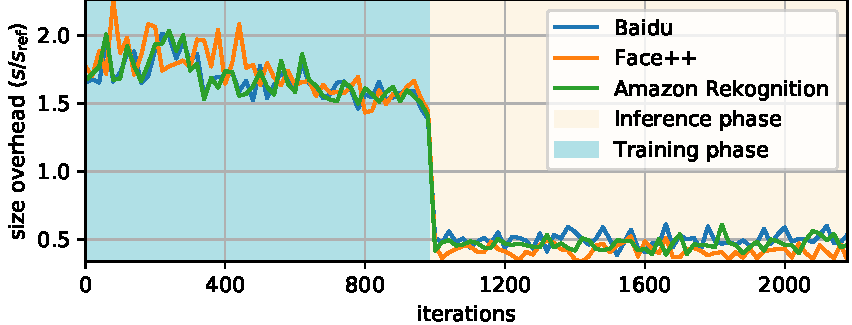
\includegraphics[width=0.8\linewidth]{figures/train_steps_new.pdf}
	\caption{Size overhead in the training and inference phase}
	\label{fig: train_steps}
	% \vspace{-0.3cm}
\end{figure}

Figure~\ref{fig: train_steps} presents the upload traffic load of the training and inference phase. To be more intuitionistic, we plot the size overhead {\color{revise2} $ \frac{\hat{s}}{\hat{s}_{\rm ref}} $} \iffalse $ \frac{s}{s_{\rm ref}} $ \fi as the $ y $-axis where {\color{revise2} $ \hat{s} $} is the real upload size of AdaCompress and {\color{revise2} $ \hat{s}_{\rm ref} $} is the benchmark upload size. Therefore $ y \geq 1 $ means that our solution uploads more data then benchmark, and $ y < 1 $ means the compression rate of AdaCompress. From Figure~\ref{fig: train_steps}, we can see that as the training procedure runs, the upload image size decreases because the RL agent learns to choose better compression quality levels to upload less data. In the training phase, to train the agent while remaining a convincing recognition result, AdaCompress has to upload the original image along with the compressed image to the cloud-end, obtaining the real result and the reward feedback. Therefore the upload traffic load is even higher than the conventional solution. But once the training phase has finished, the upload traffic load is lower than the benchmark. As shown in Figure~\ref{fig: compress_performance}, in the inference phase, AdaCompress's upload size is only 1/2 of the benchmark's. %% \\

\subsection{Size Reduction and Accuracy Performance}

\begin{figure}[!t]
	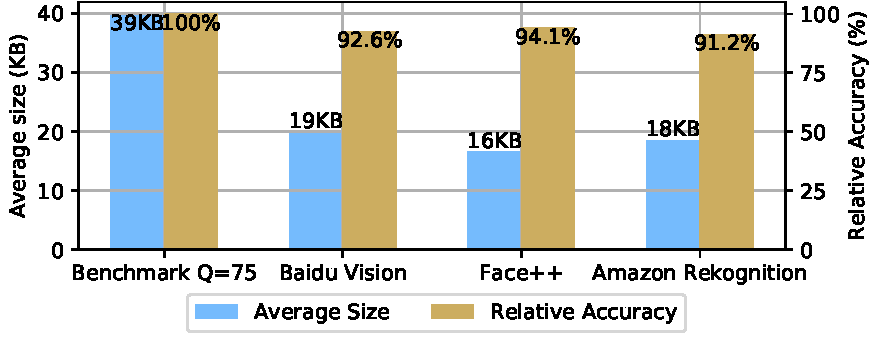
\includegraphics[width=0.8\linewidth]{figures/compress-performance.pdf}
	\caption{Average size and relative accuracy on different cloud services}
	\label{fig: compress_performance}
	% \vspace{-0.3cm}
\end{figure}

Figure~\ref{fig: compress_performance} presents the compression performance in the inference phase for each cloud service. We test AdaCompress on Face++, Baidu Vision and Amazon Rekognition. Comparing to the benchmark compression quality level, our solution can reduce the upload size by more than 1/2 for all tested cloud services, meanwhile maintain the relative accuracy that only decreases about 7\% on average, proving the efficiency of our design. %% \\

\subsection{DeepN-JPEG Comparative Experiment}

\begin{figure}[!t]
	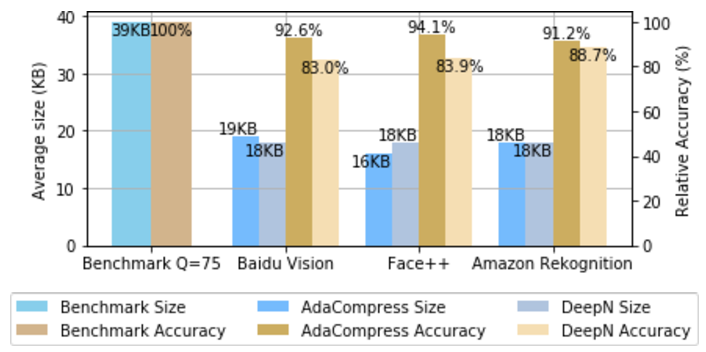
\includegraphics[width=0.8\linewidth]{figures/compare_DeepN.pdf}
	\caption{Comparative compression performance between DeepN-JPEG and AdaCompress}
	\label{fig: compare_DeepN}
	%    \vspace{-0.3cm}
\end{figure}

Figure~\ref{fig: compare_DeepN} presents a comparison performance between DeepN-JPEG and AdaCompress for each cloud service. As we can see, both DeepN-JPEG and AdaCompress cut down the upload size overhead more than 1/2. However, for all tested cloud services, AdaCompress's accuracy is higher than DeepN-JPEG's slightly. Compared with DeepN-JPEG's average accuracy is about 85\% on three cloud services, AdaCompress achieves a better average accuracy of 93\%. In a word, comparing to the DeepN-JPEG framework, AdaCompress presents a similar size reduction performance but achieving higher inference accuracy for online computer vision-based services.

\begin{figure*}[!t]
	\begin{minipage}{0.3\linewidth}
		\centerline{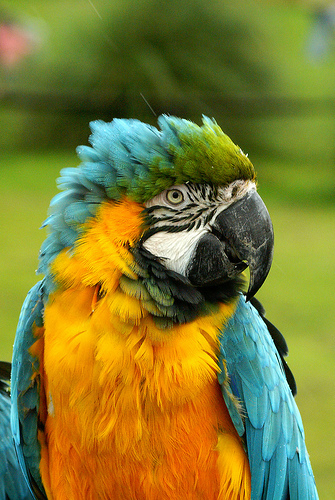
\includegraphics[width=4.0cm,trim=0 80 0 100,clip ]{figures/parrot_q75.jpeg}}
		\centerline{(1a) Origin Image (Q=75)}
		\centerline{Baidu prediction \ = \ [``parrot'']}
	\end{minipage}
	\hfill
	\begin{minipage}{0.2\linewidth}
		\centerline{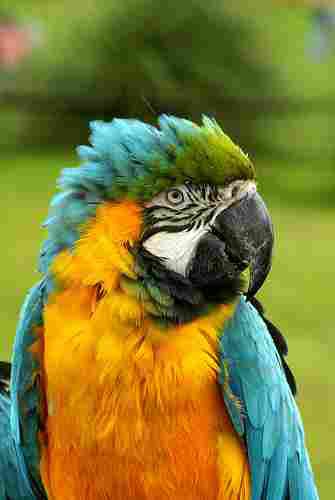
\includegraphics[width=4.0cm,trim=0 80 0 100,clip ]{figures/parrot_q15.jpeg}}
		\centerline{(1b) AdaCompress (choose Q=15)}
		\centerline{Baidu prediction \ = \ [``parrot'']}
	\end{minipage}
	\hfill
	\begin{minipage}{0.3\linewidth}
		\centerline{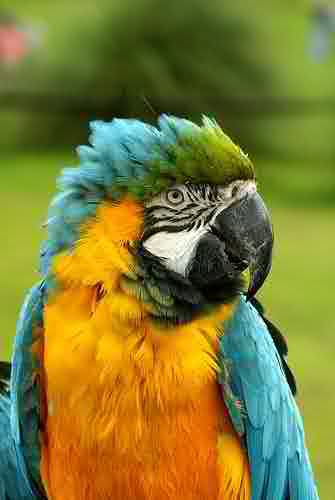
\includegraphics[width=4.0cm,trim=0 80 0 100,clip ]{figures/parrot_deepn.jpeg}}
		\centerline{(1c) DeepN-JPEG}
		\centerline{Baidu prediction \ = \ [``parrot'']}
	\end{minipage}
	
	\vfill
	\vspace{0.4cm}
	
	\begin{minipage}{0.3\linewidth}
		\centerline{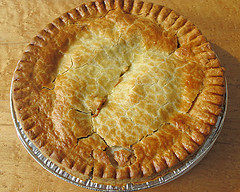
\includegraphics[width=4.0cm,trim=0 0 0 0,clip ]{figures/cake_q75.jpeg}}
		\centerline{(2a) Origin Image (Q=75)}
		\centerline{Baidu prediction \ = \ [``cake'']}
	\end{minipage}
	\hfill
	\begin{minipage}{0.2\linewidth}
		\centerline{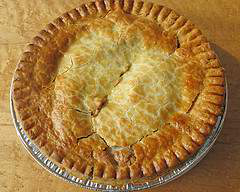
\includegraphics[width=4.0cm,trim=0 0 0 0,clip ]{figures/cake_q65.jpeg}}
		\centerline{(2b) AdaCompress (choose Q=65)}
		\centerline{Baidu prediction \ = \ [``cake'']}
	\end{minipage}
	\hfill
	\begin{minipage}{0.3\linewidth}
		\centerline{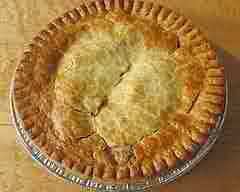
\includegraphics[width=4.0cm,trim=0 0 0 0,clip ]{figures/cake_deepn.jpeg}}
		\centerline{(2c) DeepN-JPEG}
		\centerline{Baidu prediction \ = \ [``fossil'']}
	\end{minipage}
	%	\vspace{0.2cm}
	\caption{Comparative compressed images of DeepN-JPEG and AdaCompress}
	\label{fig: compare_image}
\end{figure*}

AdaCompress compresses images in a more adaptive manner rather than DeepN-JPEG. (i.e., the explanation why AdaCompress achieves a better accuracy). As shown in Figure~\ref{fig: compare_image}, for picture 1a, compared to DeepN-JPEG, AdaCompress compresses the image at a more aggressive compression quality level of 15, reducing upload size overhead. On the contrary, for picture 2a of Figure~\ref{fig: compare_image}, DeepN-JPEG compresses the image with the same quantization table, but AdaComperss chooses a relatively higher compression quality level to preserve more details so that the backend deep learning model can still recognize the picture. Compared with DeepN-JPEG compresses all images with the same quantization table, AdaCompress chooses a low compression quality level for picture 1a and a relatively higher compression quality level for picture 2a based on the features of the input image. 

%Comparing to DeepN-JPEG, AdaCompress compresses images more adaptively for different images and cloud computer vision services to achieve higher accuracy, while maintaining a similar average upload size overhead.

Comparing to DeepN-JPEG, AdaCompress has two advantages and one disadvantage as following: %% \\    

\begin{itemize}
	
\item AdaCompress and DeepN-JPEG both decrease the upload size overhead more than 1/2, but AdaCompress maintains higher inference accuracy.

%\item DeepN-JPEG requires the original dataset information to re-design the quantization table, while AdaCompress chooses compression quality levels adaptively without any prior knowledge of the original dataset.
%\item When the scenery changes, DeepN-JPEG still compresses images with the same quantization table, while AdaCompress's \emph{inference-estimation-querying-retraining} mechanism captures the scenery change and make a more suitable compression strategy for the current scenery.
\item For different ``sceneries'' or cloud services, DeepN-JPEG compresses images with the same quantization table, while AdaCompress makes a more proper compression strategy adaptively.

%\item For different cloud services, DeepN-JPEG compresses images with the same quantization table, while AdaCompress makes a more proper compression strategy adaptively.
\item DeepN-JPEG re-designs the quantization table \emph{locally}, while AdaCompress needs to upload reference images and compressed images to the cloud-end in the training phase, leading some upload size overhead at the beginning. 
\end{itemize}

\subsection{Adaptively Cope With the Scenery Change}

To evaluate the efficiency of the \emph{inference-estimation-querying-retraining} mechanism, we feed AdaCompress with a combined dataset whose first 2000 images from FLIR Thermal images, the next 3000 images randomly sampled from ImageNet and the last 2000 images from FLIR Thermal images. We adapt AdaCompress's current RL agent to FLIR nighttime scenery by training it on the FLIR dataset, and run AdaCompress on the combined dataset, observing AdaCompress's behaviors upon the scenery changes at step 2000 and 5000. %% \\

We illustrate AdaCompress's behaviors in Figure~\ref{fig: running-retrain}. The $ x $-axis indicates steps, and the reference line indicates the scenery change. We plot AdaCompress's overall accuracy and the estimation probability $ p_{\rm est} $. At the bottom of Figure~\ref{fig: running-retrain}, we also plot the scaled upload size of AdaCompress and benchmark solution to illustrate the upload size overhead.
%with a $ \Delta $ mark on $ x $-axis

%\begin{figure}[!t]
%    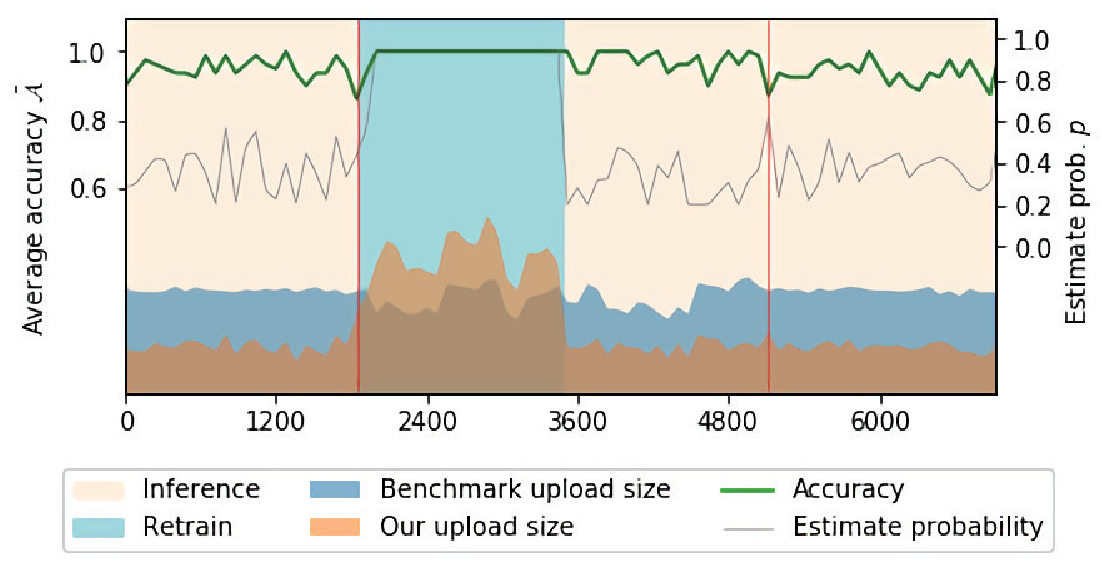
\includegraphics[width=\linewidth]{figures/running-retrain.pdf}
%    \caption{AdaCompress's reaction upon scenery change}
%%    \vspace{-0.2cm}
%    \label{fig: running-retrain}
%\end{figure}
\begin{figure}[!t]
	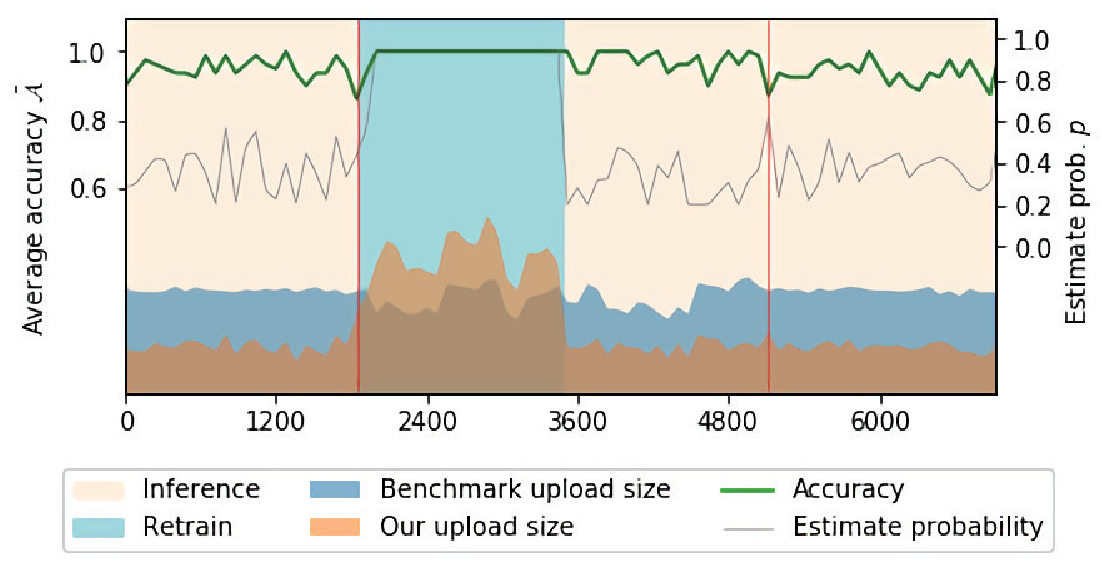
\includegraphics[width=0.8\linewidth]{figures/running-retrain.pdf}
	\caption{AdaCompress's reactions upon scenery change}
	%    \vspace{-0.2cm}
	\label{fig: running-retrain}
\end{figure}

From Figure~\ref{fig: running-retrain}, we can see that AdaCompress can adaptively update the estimation probability $ p_{\rm est} $. When the overall accuracy decreases, AdaCompress would increase the estimation probability, trying to capture the scenery change. When the overall accuracy is stable and high enough, the estimation probability $ p_{\rm est} $ decreases to reduce transmission. %% \\

Upon the first image scenery changes (i.e., night to day) shown as the first reference line in Figure~\ref{fig: running-retrain}, comparing to the earlier steps, the accuracy decreases dramatically and the estimation probability $ p_{\rm est} $ raises to determine whether the scenery changes. The accuracy keeps dropping in the following steps, indicating that the current RL agent is no more suitable for the current input scenery. At the moment, AdaCompress should switch to the model querying state and re-load a new RL agent model from the model caching library. However, there is no model except the current RL agent at that time. Therefore, AdaCompress starts to re-train at once to adapt the RL agent to the current scenery. In the re-training phase, AdaCompress uses the reference image's prediction label $ \vec{y}_{\rm ref} $ as the output result. Therefore the accuracy $ \mathcal{A} $ and $ p_{\rm est} $ are locked to 1. After finishing re-training the agent in the daytime scenery, the trained agent is cached in the model caching library. In the following steps, sometimes the accuracy decreases accidentally, and the estimation probability $ p_{\rm est} $ also raises. The accuracy is not lower than the accuracy threshold $ \mathcal{A}_0 $. Therefore the re-training phase would not be triggered again until the second image scenery changes. %% \\

Upon the second image scenery changes (i.e., day to night) shown as the second reference line in Figure~\ref{fig: running-retrain}, like the first scenery change, the accuracy decreases and $ p_{\rm est} $ raises, indicating that the current RL agent is no more suitable again. AdaCompress switches to the model querying state at once and re-loads a new RL agent model (the initial model trained on the FLIR Thermal images) from the model caching library. When using the new agent in this scenery, the accuracy stops decreasing and maintains more than the accuracy threshold, indicating the current RL agent is suitable for the current scenery.  %% \\

From Figure~\ref{fig: running-retrain}, we can also observe the upload size overhead in different phases. In the re-training phase, AdaCompress uploads more data than the conventional benchmark. But in the inference phase, AdaCompress's upload size is only half of the benchmark's. Especially once the second image scenery changes, AdaCompress achieves a low upload traffic load by re-loading a suitable RL agent model rather than re-training from scratch. %% \\

\subsection{End-to-End Latency Simulation}

Comparing to the conventional solution that uploads the image directly, in our solution, the image is passed to the RL agent firstly to estimate the compression quality level. Running this RL agent brings extra latency to the whole system. In this subsection, we evaluate the end-to-end latency. %% \\

We compute compressed file size for batches of images, and test the RL agent's inference time and the latency of uploading such compressed images. \textcolor{revise}{We respectively test the average inference latency on 1000 ImageNet images and 1000 FLIR images}, and simulate the network bandwidth as 27.64 Mbps according to the global average fixed broadband upload speed~\cite{speedtest} in Feb. 2019, to verify the end-to-end latency performance. The latency comparison is listed in Table~\ref{tab: latency-overhead}. %% \\

%We compute compressed file size for batches of images, and test the RL agent's inference time and the latency of uploading such compressed images. We test the average inference latency on 1000 ImageNet images and simulate the network bandwidth as 27.64 Mbps according to the global average fixed broadband upload speed~\cite{speedtest} in Feb. 2019, to verify the end-to-end latency performance. The latency comparison is listed in Table~\ref{tab: latency-overhead}. %% \\

\begin{table*}[!t]
{\color{revise}
	\centering
	\caption{\textcolor{revise}{Latency of edge device to cloud service}}
	\label{tab: latency-overhead}
	%     \begin{tabular}{lll}
	\resizebox{\textwidth}{!}{
	\begin{tabular}{cccccc}
		\toprule
		Dataset & Solution & Average upload size & Inference latency \
		& Transmission latency & End-to-end latency \\ \midrule
		ImageNet & Benchmark & 42.68 KB & 0 ms & 12.35 ms & 12.35 ms \\
		ImageNet & AdaCompress & 18.64 KB & 2.09 ms & 5.34 ms & 7.43 ms \\
		FLIR & Benchmark & 44.66 KB & 0 ms & 12.93 ms & 12.93 ms \\
 		FLIR & AdaCompress & 17.07 KB & 2.03 ms & 4.94 ms & 6.97 ms \\ \bottomrule
	\end{tabular}}
	% \vspace{-0.5cm}
}
\end{table*}
%\begin{table*}[!t]
%	\centering
%	\caption{Latency between image upload and inference result feedback}
%	\label{tab: latency-overhead}
%	%     \begin{tabular}{lll}
%	\begin{tabular}{ccc}
%		\toprule
%		& Benchmark & AdaCompress  \\ \midrule
%		Average upload size          & 42.68 KB  &  18.46 KB            \\
%		Inference latency    & 0 s       & 2.09 ms          \\
%		Transmission latency & 12.35 ms       & 5.34 ms          \\
%		Overall latency      & 12.35 ms       & 7.43 ms          \\ \bottomrule
%	\end{tabular}
%	% \vspace{-0.5cm}
%\end{table*}

Our solution brings in inference latency to the end-to-end latency, but the transmission latency is low by reducing the upload file size. In today's network architecture where the edge infrastructure's computational power is increasing significantly~\cite{satyanarayanan2017emergence,hu2015mobile}, we can use the computing power of the edge infrastructure in exchange for the reduction of upload traffic load and transmission latency. \textcolor{revise}{Compared with the benchmark solution, our solution effectively reduces the end-to-end latency on both ImageNet and FLIR dataset.} %% \\

\subsection{\textcolor{revise}{Overall Memory and Latency Overhead}}

\subsubsection{\textcolor{revise}{Memory Overhead:}}
\textcolor{revise}{The memory overhead is divided into two parts: the static occupied memory space and dynamic memory usage. Firstly, the static occupied memory space is the memory of the model's size. We use Keras to construct and save MobileNetV2 and the RL agent. We check file size of the saved model as the model's size. A RL agent model's size is 1 MB, and the feature extractor MobileNetV2's size is 8.9 MB. The model caching library stores the most recent five RL agents. The overall memory of the model's size is at most 13.9 MB. Secondly, the dynamic memory usage is the memory usage during AdaCompress runs. The overall memory usage mainly includes the memory buffer of transitions and the memory usage caused by the RL agent and feature extractor. When caching transitions of 1000 images in the memory buffer, it occupies about 500 KB. We use Psutil to measure the peak memory usage during AdaCompress runs. The peak memory usage is about 367 MB. Thirdly, in real-world edge-application scenarios, common edge infrastructures have enough memory to deploy this algorithm, such as Raspberry Pi 4 Model B's \cite{Raspberry-Pi} memory is 2/4/8 GB, and Huawei Atlas 500 edge station's memory is 4/8 GB.}

\subsubsection{\textcolor{revise}{Training and Re-loading Latency:}}
\textcolor{revise}{Although AdaCompress can be highly efficient to run on today's edge infrastructures, it would cause extra latency overhead, such as training and re-loading latency. In this subsection, we evaluate the latency overhead.}

%\begin{table*}[!t]
%	\centering
%	\caption{Time cost of training}
%	\label{tab: training-time}
%		\begin{tabular}{cccc}
%			\toprule
%			Dataset & Number of training images & Time cost & Real time cost \\ \midrule
%			ImageNet & 898 & 15.86 min & 7.89 min \\
%			FLIR & 910 & 15.63 min & 7.85 min \\ \bottomrule
%	\end{tabular}
%	% \vspace{-0.5cm}
%\end{table*}

\textcolor{revise}{In our experiments, the convergence condition of training is that the recent average accuracy over 0.8 meanwhile the recent average reward over 0.45. The experiment results show the number of training images is 898 and 910 on ImageNet and FLIR, respectively. The time cost mainly depends on the frequency of sending images and the inference speed of the cloud service. If the end-user sends images continuously, and cloud service's inference speed is about 10 images per second, the time costs are 197.3s and 200.8s on ImageNet and FLIR, respectively. In the training phase, we need to upload reference images and compressed images. We consider the time cost of uploading reference images and obtaining the feedbacks as the benchmark latency. If we minus this benchmark latency, the real training time cost is not over 100s. It is worth to spend such upload size overhead and time cost at the beginning when we need to infer thousands of images.}

%And the training time respectively is 15.36 min and 15.63 min on ImageNet and FLIR.

\textcolor{revise}{The \emph{inference-estimation-querying-retraining} mechanism would either re-load or re-train a RL agent intelligently when capturing the scenery change. The re-training time cost is similar to the training time cost which is described above. The latency of re-loading a RL agent model is about 1.85s. To \emph{reduce} this latency, we use another process to re-load the model in our experiments. The mechanism still uses the old RL agent to choose a compression quality level before the re-loading process has finished.}
